% -----------------------------------------------------------------------------
%   Arquivo: ./02-elementos-textuais/trabalhosRelacionados.tex
% -----------------------------------------------------------------------------

\chapter{Aprendizado de Máquina}
\label{chap:MachineLearning}

\section{Formulação e Caracterização do Aprendizado de Máquina}

Nos primórdios da inteligência artificial, pesquisadores foram capazes de resolver problemas que são intelectualmente difíceis para os seres humanos, mas relativamente simples para os computadores. Exemplo disso são os problemas que podem ser descritos por uma sequência de regras ou que podem ser solucionados por operações matemáticas \cite{Goodfellow-et-al-2016}.

A dificuldade surgiu para fazer com que os computadores fossem capazes de resolver tarefas fáceis para os humanos, mas difíceis de serem descritas de forma algorítmica, como reconhecer escrita, identificar rostos em imagens ou ainda definir regras de decisão de forma autônoma \cite{Goodfellow-et-al-2016}.

Eis que surgiu o campo de Aprendizado Máquina, uma alternativa que permitia computadores aprender por exemplo e não por regras. Ao reunir o conhecimento da experiência, esta abordagem evita a necessidade de operadores humanos especificar formalmente todo o conhecimento que o computador precisa. Isso ocorre através da combinação do aprendizado de conceitos simples, em formato pré-definido, combinados de forma hierárquica para formar um aprendizado de conceitos complicados \cite{Goodfellow-et-al-2016}.

Segundo \citeonline{Cherkassky2007}, o processo de aprendizado é definido como a estimação de uma relação ou estrutura, previamente desconhecida, entre entrada e saída. Segundo o autor, o processo de aprendizado normalmente envolve três componentes \ref{fig:MLFormulation} : o \textit{Gerador} de amostras, um \textit{Sistema} que gera as saídas reais e o \textit{Aprendizado de Máquina} que estima a relação desconhecida entre entrada e saída. 

\begin{figure}[!htb]
	\centering
	\caption{Formulação do Aprendizado} 
	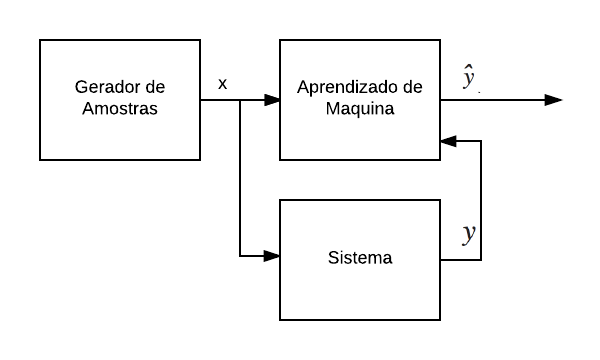
\includegraphics[width=0.8\textwidth]{./04-figuras/MLForm.png}
	\label{fig:MLFormulation}
\end{figure}

\citeonline{Cherkassky2007} explica que o \textit{Gerador} produz aleatoriamente, com distribuição de probabilidade $p(x)$, vetores $x \in {\mathbb {R}} ^{n}$, que são as características. O \textit{Sistema} é capaz de produzir, com probabilidade $p(y | x)$, saídas $y = f(x) + \epsilon$ em que $\epsilon$ é um ruido branco de $\mu = 0$. De forma geral, o \textit{Aprendizado de Máquina} é capaz de implementar uma função $\hat{y} = f(x, \omega)$, $\omega \in \Omega$, em que $\Omega$ é conjunto de parâmetros da função $f$.

O aprendizado de máquinas clássico diz respeito à aprender pelo exemplo, que é definido como um conjunto de dados, previamente obtidos pelo \textit{Gerador} e \textit{Sistema}, composto por variáveis quantitativas e qualitativas que são características do problema. Na situação onde existe uma variável resposta, o aprendizado é chamado de supervisionado, na situação onde essa variável não existe, o problema é definido como aprendizado não supervisionado. A figura \ref{fig:MLProblems} ilustra essa taxonomia, bem como algumas de suas sub-divisões.


\begin{figure}[!htb]
	\centering
	\caption{Problemas de Aprendizado de Máquina} 
	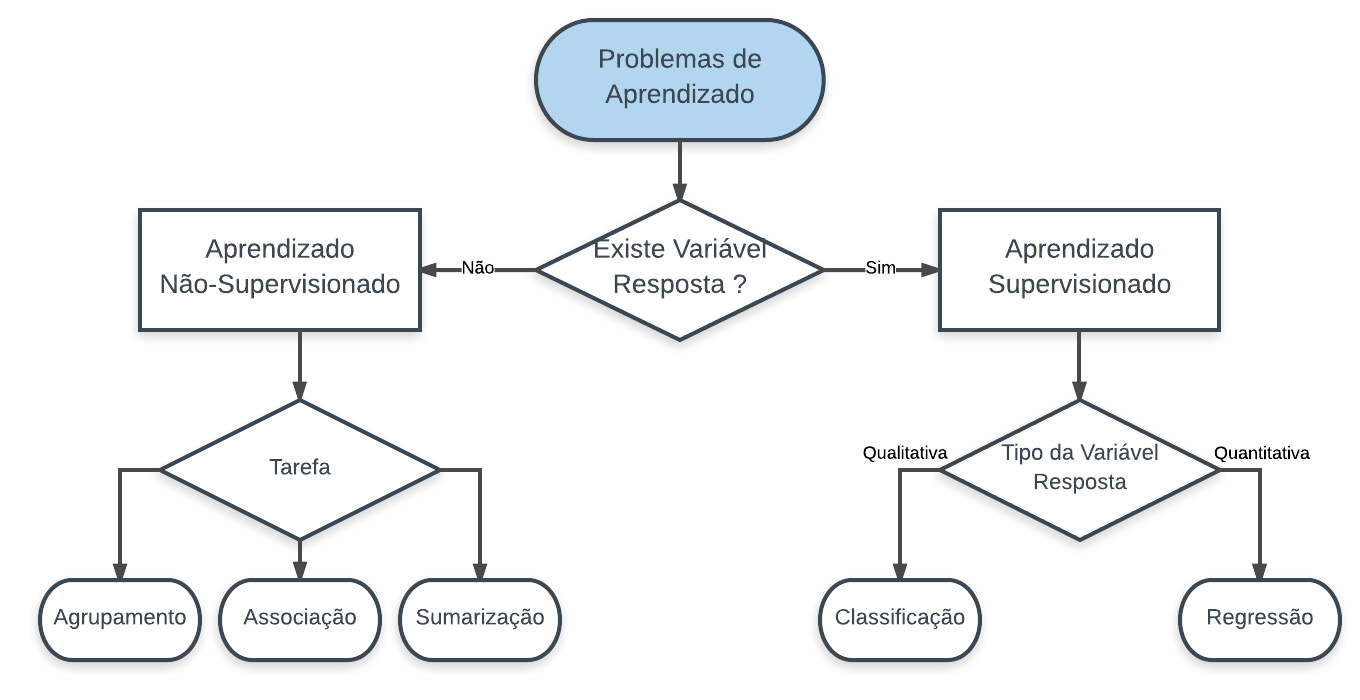
\includegraphics[width=0.8\textwidth]{./04-figuras/MLProblems.png}
	\label{fig:MLProblems}
\end{figure}
\section{Aprendizado Supervisionado}

No aprendizado supervisionado, o objetivo é prever o valor de uma variável resultado com base em variáveis características. Na situação que a variável resposta é quantitativa, o problema é considerado como uma tarefa de regressão. Quando essa variável resposta é quantitativa, a tarefa é chamada de classificação.

De acordo com \citeonline{Cherkassky2007}, existem duas interpretações para o problema de aprendizado : identificação e imitação. A interpretação escolhida para fundamentar esse trabalho é a de imitação, descrita por \citeonline{Vapnik1971}.

O objetivo do aprendizado é encontrar uma função $f(x, \omega)$ que aproxima, da melhor forma possível, a saída $y$ do Sistema. Para formular esse problema matematicamente, \citeonline{Cherkassky2007}, assume-se pares de características e respostas, $(x_i, y_i)$ em que $i = (1, 2, ..., n)$ e $ n \in \mathbb {N}$, 



\subsection{Problemas de Classificação}
\subsection{Problemas de Regressão}

\section{Aprendizado Não Supervisionado}

\section{Métricas de Aprendizado}
